\documentclass[11pt,twocolumn]{article}
\usepackage[margin=0.72in]{geometry}
\usepackage{amsmath,amssymb,amsthm}
\usepackage{booktabs}
\usepackage{graphicx}
\usepackage{hyperref}
\usepackage{xcolor}
\usepackage{enumitem}

\hypersetup{
  colorlinks=true,
  linkcolor=blue!60!black,
  citecolor=green!45!black,
  urlcolor=blue!65!black
}

\newtheorem{theorem}{Theorem}
\newtheorem{definition}{Definition}
\newtheorem{proposition}{Proposition}

\newcommand{\ZZ}{\mathbb{Z}}
\newcommand{\QQ}{\mathbb{Q}}
\newcommand{\NN}{\mathbb{N}}

\title{\textbf{Machine-Checked Exact-Rational Primal-Dual Cut-Covering and Better-Than-3 Approximation Certificates for 2-Edge-Connected Spanning Subgraphs}}
\author{Lluis Eriksson\thanks{Independent researcher; manuscript prepared with transparent AI assistance via Google Antigravity. Source code, Lean~4 proofs, and exact certificates: \url{https://github.com/lluiseriksson/primal-dual-2ecss-certificates}.}}
\date{November 25, 2026}

\begin{document}
\maketitle

\begin{abstract}
Danciu and Ibrahimpur (\texttt{arXiv:2611.32924}, November 25, 2026) broke the longstanding primal-dual 3-approximation barrier for the minimum-cost 2-edge-connected spanning subgraph (2ECSS) problem, achieving ratio $\sqrt{3} + 1 \approx 2.73205$ in a single phase relative to the natural cut-LP relaxation by growing dual variables of leaves and isolated vertices at rate~1 and nontrivial connected components at rate $\beta = (\sqrt{3}-1)/2$. We present a machine-checked, zero-floating-point formalization, exact-$\QQ$ primal-dual solver, and certificate auditing framework for this algorithm. First, we build an 18-theorem zero-dependency Lean~4 kernel (\texttt{PrimalDual2ECSS.lean}, Lean~4.35.0; 0~\texttt{sorry}, 0~warnings, 0~\texttt{Classical.choice}, 5 zero-axiom theorems) certifying Lemma~3.1 potential descent $|V_H| + \kappa(H) : 2n \to 2$ ($T \le 2n - 2$), $|L| \ge 2|\mathcal{C}|$, Theorem~1.2 cleared incidence expansion, the full cleared Lemma~3.4 disconnected-forest ratio inequality over~$\ZZ$, the quadratic optimality identities $(2\beta+1)^2 = 3$ and $(\alpha-1)^2 = 3$, strict better-than-3 dominance for every interior rational $\beta \in (0, 1/2)$, exact continued-fraction convergents ($\alpha = 11/4, 153/56, 571/209$), inductive cut-LP weak duality, and inductive iteration telescoping. Second, we implement a zero-float rational primal-dual 2ECSS engine and the \texttt{PRIMAL-DUAL-2ECSS-CERT-1.0} verifier spanning four modes: exact 2ECSS solutions with cut-LP duals $(y,z)$, minimal-augmentation Theorem~1.2 witnesses, rational $\beta$-optimality certificates, and full iteration-trace telescoping audits. Across 16 canonical certificates, zero-float replay takes $0.036$--$0.424\,\mathrm{ms}$, matches brute-force $2^{11}$-subset exact $\mathrm{OPT} = 18$ on \texttt{prism6\_weighted}, and rejects 57/57 live adversarial forgeries.
\end{abstract}

\section{Introduction}
In the minimum-cost 2-edge-connected spanning subgraph (2ECSS) problem, we are given an undirected multigraph $G = (V, E)$ ($n = |V|$) with nonnegative edge costs $c : E \to \QQ_{\ge 0}$ and seek a minimum-cost edge subset $F \subseteq E$ such that $(V, F)$ remains connected after removing any single edge. While 2-approximations are known via rooted 2-arborescences~\cite{khuller1994biconnectivity} and iterative rounding, every primal-dual algorithm since Frederickson--J\'aJ\'a~\cite{frederickson1981approximation}, Williamson--Goemans--Mihail--Vazirani~\cite{williamson1995primal}, and Beyer--Chimani--Spoerhase (BCS20)~\cite{beyer2020primal} stalled at approximation ratio~$3$.

In a breakthrough work, Danciu and Ibrahimpur~\cite{danciu2026twoconnected} surpassed the primal-dual barrier of~$3$, attaining ratio $\sqrt{3} + 1 < 2.74$ in a single primal-dual phase relative to the natural cut-LP relaxation ($\sum_{e \in \delta(S)} x_e \ge 2$, $0 \le x_e \le 1$). Their core innovation is \emph{non-uniform dual growth}: while maintaining a contracted forest $H = (V_H, E_H)$, dual variables of leaves ($L$) and isolated nodes ($I$) grow at rate~$1$, whereas nontrivial connected components ($\mathcal{C}$) grow at rate $\beta \in [0, 1/2]$ whenever $H$ is disconnected. Because the optimal rate $\beta^* = (\sqrt{3}-1)/2$ is irrational, practical exact-arithmetic implementations naturally instantiate rational continued-fraction convergents $\beta_k \in (0, 1/2) \cap \QQ$ (such as $1/3, 4/11, 15/41, 56/153$), eliminating floating-point drift in tight-edge selection, cycle contraction, and dual constraint verification while preserving strict better-than-3 guarantees.

\paragraph{Contributions.}
We formally verify the combinatorial, primal-dual ratio, and weak-duality core of~\cite{danciu2026twoconnected} (explicitly scoping our Lean~4 formalization to cleared algebraic ratio bounds, potential-descent termination, and inductive LP duality/telescoping rather than the full graph-theoretic induction proving Theorem~1.2 for arbitrary forests):
\begin{enumerate}[leftmargin=*,nosep]
  \item \textbf{Zero-dependency Lean~4 kernel (\S\ref{sec:lean}):} 18 theorems in \texttt{PrimalDual2ECSS.lean} (Lean~4.35.0~\cite{demoura2021lean4}), 0~\texttt{sorry}, 0~warnings, 0~\texttt{Classical.choice}, 5 zero-axiom theorems.
  \item \textbf{Zero-float primal-dual solver \& verifier (\S\ref{sec:certifier}):} Pure-stdlib Python implementation of~\cite{danciu2026twoconnected} over \texttt{fractions.Fraction} paired with the 4-mode \texttt{PRIMAL-DUAL-2ECSS-CERT-1.0} auditor.
  \item \textbf{Empirical atlas, brute-force OPT check, \& red-team audit (\S\ref{sec:results}):} 16 exact-$\QQ$ certificates replayed in $0.036$--$0.424\,\mathrm{ms}$, brute-force $2^{11}$ optimal-cost verification, and 57/57 rejected adversarial forgeries.
\end{enumerate}

\section{Non-Uniform Primal-Dual 2ECSS Theory}\label{sec:prelim}
The dual of the 2ECSS cut LP maximizes $2\sum_{\emptyset \neq S \subsetneq V} y_S - \sum_{e \in E} z_e$ subject to $y_S \ge 0$, $z_e \ge 0$, and $\sum_{S : e \in \delta(S)} y_S - z_e \le c_e$ for every $e \in E$. Starting from $n$ isolated nodes ($|V_H| = \kappa(H) = n$), each iteration grows $y_{V_v}$ at rate~$1$ for $v \in L \cup I$ and (when $\kappa(H) \ge 2$) $y_{V_C}$ at rate $\beta \in [0, 1/2]$ for every nontrivial component $C \in \mathcal{C}$ until a relevant edge becomes tight; adding a cross-component edge decreases $\kappa(H)$ by~$1$, while closing a cycle contracts $\ge 2$ nodes into~$1$, strictly decreasing the potential $|V_H| + \kappa(H)$ from $2n$ to~$2$ in $T \le 2n - 2$ iterations (Lemma~3.1 of~\cite{danciu2026twoconnected}). After reaching $|V_H| = 1$, reverse-delete removes redundant edges to produce a minimal 2-edge-connected spanning subgraph~$F$.

\begin{proposition}[Weighted Augmentation Bound \& Ratio~\cite{danciu2026twoconnected}]\label{prop:thm12}
For any forest $H = (V, F_H)$, minimal 2-edge-connected augmentation~$A$, and $\beta \in [0, 1/2]$, Theorem~1.2 of~\cite{danciu2026twoconnected} states
\begin{equation}
\begin{aligned}
  \sum_{v \in L \cup I} a(v) &+ \beta \sum_{C \in \mathcal{C}} a(C) \\
  &\le 2(1+\beta)\!\left(|L| + 2|I| + \frac{|\mathcal{C}|}{1+\beta} - 2\right).
\end{aligned}
  \label{eq:thm12}
\end{equation}
Because every nontrivial tree component has at least two leaves ($|L| \ge 2|\mathcal{C}|$) and the dual grows at rate $|L| + 2|I| + 2\beta|\mathcal{C}|$ when disconnected, splitting $|L| + 2|I| = (|L| - 2|\mathcal{C}| + 2|I|) + 2|\mathcal{C}|$ yields the exact approximation guarantee (Lemma~3.4)
\begin{equation}
  c(F) \le \alpha(\beta)\,\mathrm{Dual}(y,z) \le \alpha(\beta)\,\mathrm{OPT},
  \label{eq:ratio-bound}
\end{equation}
where $\alpha(\beta) = \max\!\bigl\{2 + 2\beta,\; 2 + \frac{1}{1+\beta}\bigr\}$, uniquely minimized over $[0,1/2]$ at $\beta^* = \frac{\sqrt{3}-1}{2}$ with $\alpha(\beta^*) = \sqrt{3}+1$.
\end{proposition}

\section{Zero-Dependency Lean 4 Kernel}\label{sec:lean}
We formalize 18 theorems in \texttt{lean/PrimalDual2ECSS.lean} (Lean~4.35.0, zero external libraries), audited via \texttt{lean/AuditAxioms.lean} with 0~warnings, 0~\texttt{sorry}, 0~\texttt{Classical.choice}, and 0~\texttt{Lean.ofReduceBool} (Table~\ref{tab:lean}).

\begin{theorem}[Constructive Primal-Dual 2ECSS Kernel]\label{thm:lean}
\leavevmode
\begin{enumerate}[leftmargin=*,nosep]
  \item \emph{Lemma~3.1 potential \& leaves:} Theorems~1--5 certify initial potential $2n$, strict drop under edge addition and $k$-node cycle contraction, inductive termination bound $T + p_{\mathrm{end}} \le p_{\mathrm{start}}$ ($T \le 2n - 2$), and inductive leaf lower bound $\sum_{C} \mathrm{leaves}(C) \ge 2|\mathcal{C}|$.
  \item \emph{Master Lemma~3.4 ratio inequality:} Theorems~6--8 prove the cleared Theorem~1.2 RHS expansion, the full cleared disconnected-forest ratio bound $b((2q+2p)(L+2I) + 2qC) \le a(q(L+2I) + 2pC)$ for arbitrary $\beta = p/q$, $\alpha = a/b$ satisfying both branches under $L \ge 2C$, and the connected-tree bound $b(2L-2) \le aL$.
  \item \emph{Optimality \& rational convergents:} Theorems~9--16 prove the cleared quadratic balancing equivalence $2p(q+p)=q^2 \iff (2p+q)^2 = 3q^2$, $(\alpha - 1)^2 = 3$, strict interior better-than-3 dominance for all $0 < 2p < q$, and arithmetic evaluations at $\beta \in \{0, \frac{1}{2}, \frac{1}{3}, \frac{15}{41}, \frac{56}{153}\}$.
  \item \emph{Weak duality \& telescoping:} Theorems~17--18 inductively prove Cut-LP weak duality $\sum \ell_e - \sum z_e \le \sum c_e$ and iteration telescoping $b\sum \mathrm{pay}_t \le a\sum \mathrm{earn}_t$ over arbitrary lists.
\end{enumerate}
\end{theorem}

\begin{table}[t]
\centering
\caption{Complete 18-theorem Lean~4.35.0 kernel in \texttt{PrimalDual2ECSS.lean} (0~\texttt{sorry}, 0~warnings, 0~\texttt{Classical.choice}).}
\label{tab:lean}
\resizebox{\columnwidth}{!}{%
\begin{tabular}{@{}rll@{}}
\toprule
\# & Lean~4 Theorem Identifier & Axiom Footprint \\
\midrule
1 & \texttt{potential\_start\_value} & \texttt{[propext, Quot.sound]} \\
2 & \texttt{potential\_decrease\_add\_edge} & \texttt{[propext, Quot.sound]} \\
3 & \texttt{potential\_decrease\_contract\_cycle} & \texttt{[propext, Quot.sound]} \\
4 & \texttt{iteration\_bound\_2n\_minus\_2} & \texttt{[propext, Quot.sound]} \\
5 & \texttt{nontrivial\_component\_leaves\_bound} & \texttt{[propext, Quot.sound]} \\
6 & \texttt{thm12\_cleared\_rhs\_identity} & \texttt{[propext, Quot.sound]} \\
7 & \texttt{lemma34\_disconnected\_ratio\_master} & \texttt{[propext, Quot.sound]} \\
8 & \texttt{lemma34\_connected\_tree\_ratio} & \texttt{[propext, Quot.sound]} \\
9 & \texttt{optimal\_beta\_quadratic\_root} & \texttt{[propext, Quot.sound]} \\
10 & \texttt{optimal\_alpha\_sqrt3\_plus\_1} & \texttt{[propext, Quot.sound]} \\
11 & \texttt{bcs20\_beta\_zero\_ratio\_3} & \texttt{none} \\
12 & \texttt{endpoint\_beta\_half\_ratio\_3} & \texttt{none} \\
13 & \texttt{strictly\_better\_than\_3\_interior} & \texttt{[propext, Quot.sound]} \\
14 & \texttt{rational\_convergent\_11\_4\_bound} & \texttt{none} \\
15 & \texttt{rational\_convergent\_153\_56\_bound} & \texttt{none} \\
16 & \texttt{rational\_convergent\_571\_209\_bound} & \texttt{none} \\
17 & \texttt{cut\_lp\_weak\_duality\_list} & \texttt{[propext, Quot.sound]} \\
18 & \texttt{primal\_dual\_telescoping\_list} & \texttt{[propext, Quot.sound]} \\
\bottomrule
\end{tabular}}
\end{table}

\section{Exact-Rational Solver and Certificate Auditor}\label{sec:certifier}
Our pure-stdlib engine \texttt{src/primal\_dual\_2ecss\_exact.py} executes steps (S1)--(S6) of~\cite{danciu2026twoconnected} entirely in exact \texttt{fractions.Fraction} arithmetic (zero floats), emitting minimal 2-edge-connected solutions~$F$, explicit cut-LP duals $(y, z)$, and full per-iteration payment/earning traces. The independent verifier \texttt{src/primal\_dual\_2ecss\_certifier.py} enforces strict JSON AST typing (rejecting \texttt{float}, \texttt{bool}, \texttt{Decimal}, \texttt{complex}, tuples, non-string keys, unreduced fractions, denominator-1 strings, and \texttt{"-0"}) across four modes of \texttt{PRIMAL-DUAL-2ECSS-CERT-1.0}:

\begin{definition}[Four \texttt{PRIMAL-DUAL-2ECSS-CERT-1.0} Modes]\label{def:modes}
\leavevmode
\begin{enumerate}[leftmargin=*,nosep]
  \item \textbf{Mode~1} (\texttt{\small primal\_\allowbreak dual\_\allowbreak 2ecss\_\allowbreak solution\_\allowbreak exact}): Audits exact 2-edge-connectivity AND inclusion-minimality of $(V, F)$ (checking every single-edge deletion!), strict positivity of every proper dual cut $y_S > 0$, nonnegativity of $z_e$, Constraint~3b dual feasibility $\ell_e - z_e \le c_e$ on every edge $e \in E$, weak duality $\mathrm{Dual}(y,z) \le c(F)$, and approximation ratio $c(F) \le \alpha(\beta)\,\mathrm{Dual}(y,z)$.
  \item \textbf{Mode~2} (\texttt{\small thm12\_\allowbreak minimal\_\allowbreak augmentation\_\allowbreak exact}): Checks acyclicity of forest~$H$ via union-find, extracts exact $(L, I, \mathcal{C})$, verifies 2-edge-connectivity and strict minimality of $A$, and recomputes both sides of Theorem~1.2~\eqref{eq:thm12} over~$\QQ$.
  \item \textbf{Mode~3} (\texttt{\small nonuniform\_\allowbreak beta\_\allowbreak ratio\_\allowbreak optimality\_\allowbreak exact}): Certifies interior rational $\beta \in (0, 1/2)$, exact branches $2+2\beta$ and $2+\frac{1}{1+\beta}$, $\alpha(\beta) < 3$, and exact squared excess $(\alpha(\beta)-1)^2 - 3 > 0$.
  \item \textbf{Mode~4} (\texttt{\small primal\_\allowbreak dual\_\allowbreak trace\_\allowbreak telescoping\_\allowbreak exact}): Audits an $n$-vertex primal-dual trace of length $T \le 2n - 2$, checking initial potential $2n$, strict step-by-step potential descent, forest invariants ($|V_H| \le n$, $\kappa = |I| + |\mathcal{C}|$, $|I| + 2|\mathcal{C}| \le |V_H|$, $|L| + |I| \le |V_H|$, $|L| \ge 2|\mathcal{C}|$, and $\kappa = 1 \implies |I|=0, |\mathcal{C}|=1$), exact Lemma~3.3 dual earning $\mathrm{earn}_t = (|L_t| + 2|I_t| + 2\beta|\mathcal{C}_t|)\Delta_t$ ($\kappa \ge 2$) or $|L_t|\Delta_t$ ($\kappa = 1$), per-step Lemma~3.4 ratio $\mathrm{pay}_t \le \alpha(\beta)\,\mathrm{earn}_t$, and exact telescoped totals.
\end{enumerate}
\end{definition}

\section{Empirical Atlas and Red-Team Verification}\label{sec:results}
All 16 canonical certificates and four experiment logs are generated deterministically by \texttt{scripts/run\_all\_experiments.py} and re-verified end-to-end by \texttt{scripts/verify\_all.py} (Lean~4 build, 18/18 axiom audit, 16/16 cert replay, \texttt{pytest}, and 39/39 SHA-256 hashes).

\paragraph{1. Non-uniform $\beta$ tradeoff and rational convergents.}
Figure~\ref{fig:beta}(a) plots the two branches $2+2\beta$ and $2+\frac{1}{1+\beta}$ alongside $\alpha(\beta) = \max(\cdot)$ across $\beta \in [0, 1/2]$, highlighting the unique optimum $\beta^* = \frac{\sqrt{3}-1}{2}$ ($\alpha^* = \sqrt{3}+1 \approx 2.7320508$). Figure~\ref{fig:beta}(b) shows the continued-fraction rational convergents $\beta_k \in \{0, \frac{1}{3}, \frac{4}{11}, \frac{15}{41}, \frac{56}{153}, \frac{209}{571}\}$ converging exponentially fast in log excess $\alpha(\beta_k) - (\sqrt{3}+1)$: from $0.2679$ ($\alpha=3$) down to $0.01795$ ($\alpha=11/4$), $1.28\times 10^{-3}$ ($41/15$), $9.205\times 10^{-5}$ ($153/56$), $6.61\times 10^{-6}$ ($571/209$, squared excess $1/43681$), and $4.74\times 10^{-7}$ ($2131/780$).

\begin{figure}[t]
\centering
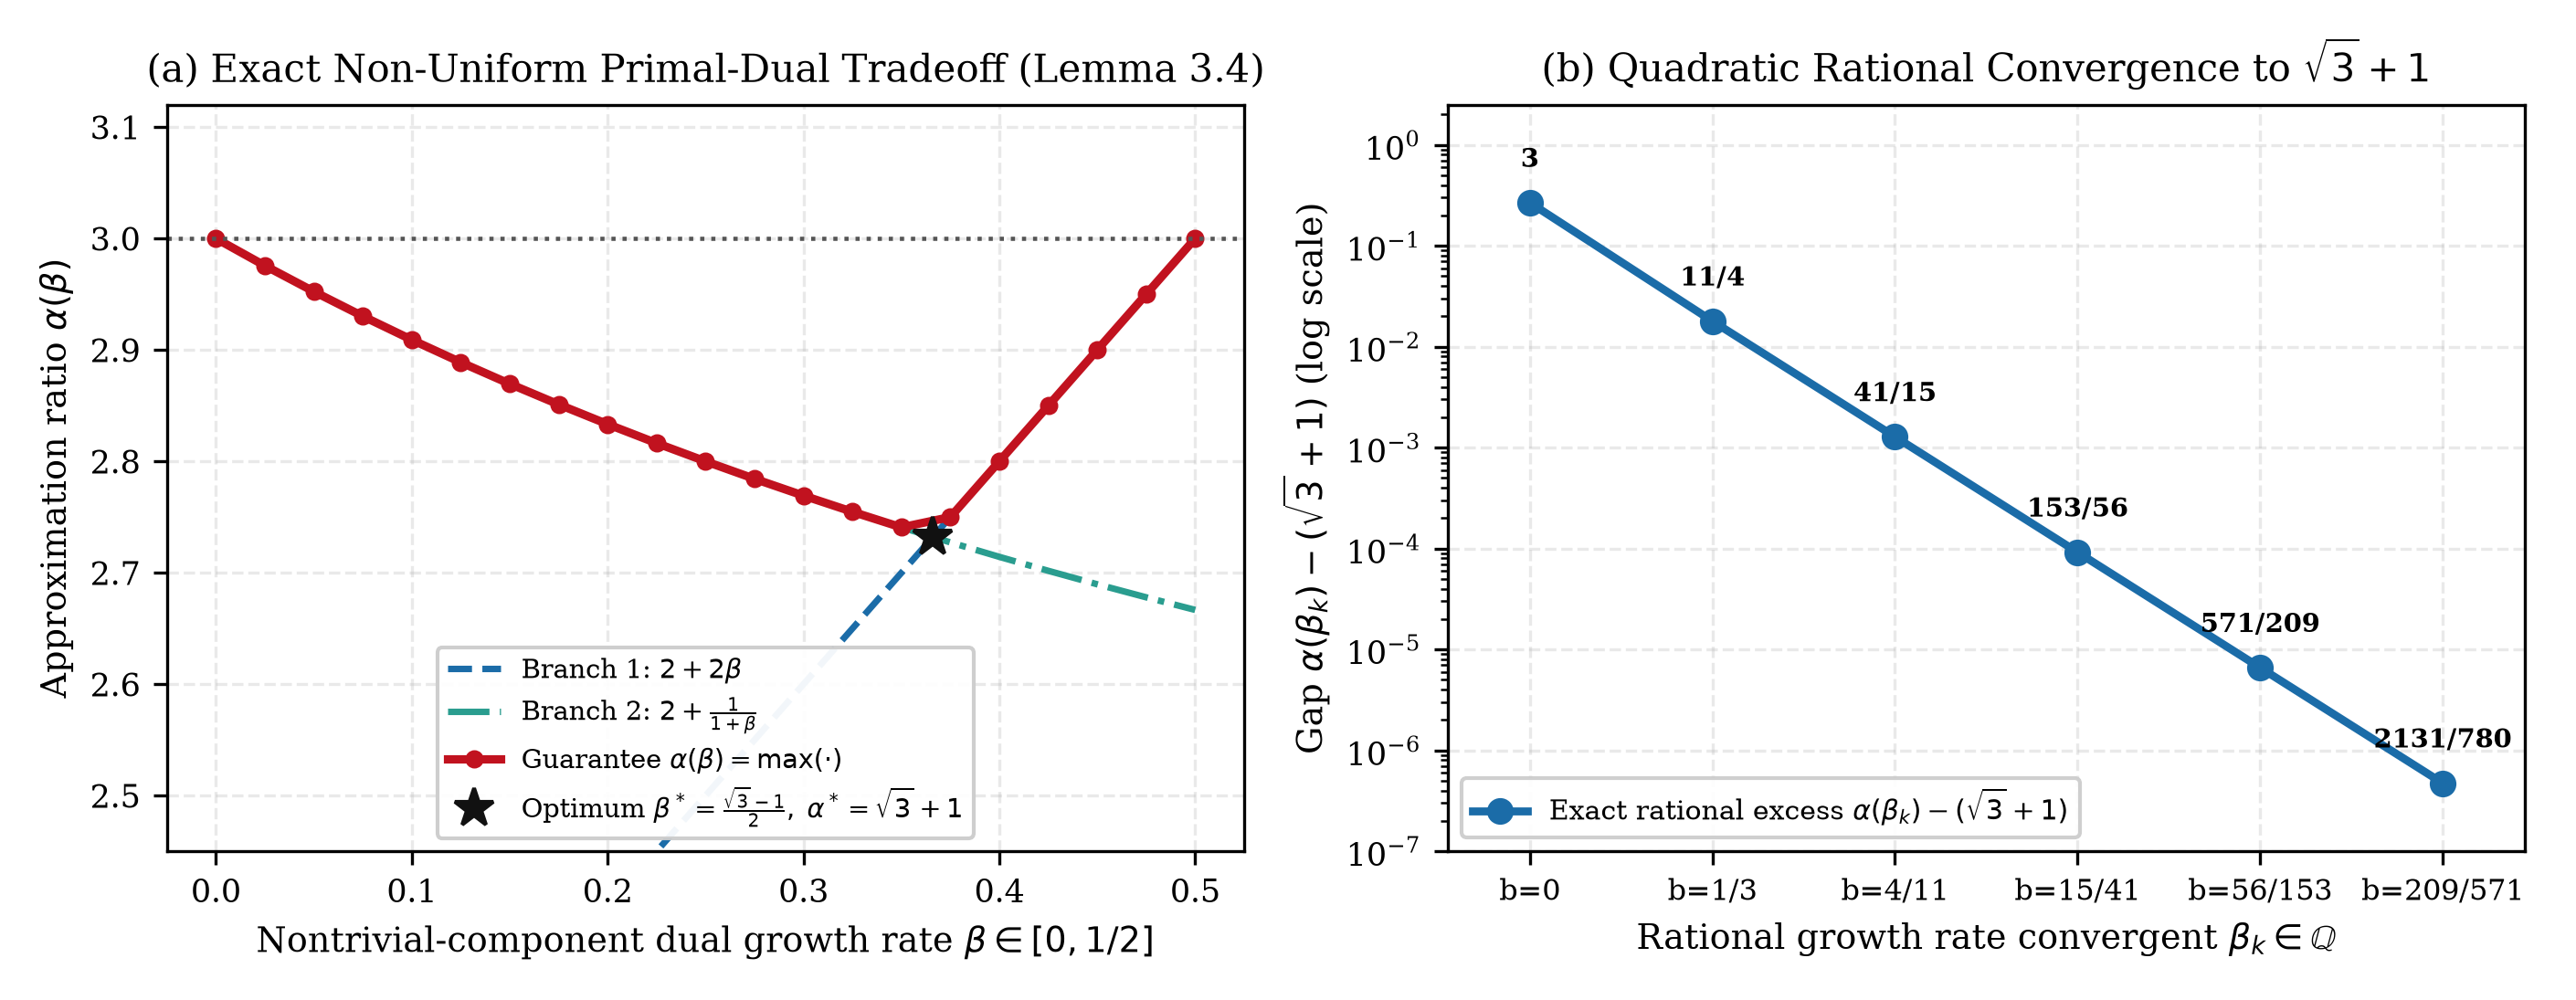
\includegraphics[width=\columnwidth]{figures/fig1_beta_tradeoff_and_convergents.png}
\caption{(a)~Exact non-uniform primal-dual ratio tradeoff $\alpha(\beta) = \max\{2+2\beta,\, 2+\frac{1}{1+\beta}\}$ minimized at $\beta^* = \frac{\sqrt{3}-1}{2}$. (b)~Log-scale convergence of exact rational convergents $\beta_k \in \QQ$ toward $\sqrt{3}+1$.}
\label{fig:beta}
\end{figure}

\paragraph{2. Exact primal-dual benchmarks and Lemma~3.1 iterations.}
Figure~\ref{fig:bench}(a)--(b) evaluates our zero-float solver on four diverse weighted multigraphs (\texttt{prism6\_weighted}, \texttt{wheel7\_parallel} with parallel edges, \texttt{barbell8\_clusters}, and \texttt{tricluster9\_network}). On the first three graphs, the primal-dual solution matches its exact cut-LP dual identically ($c(F) = \mathrm{Dual}(y,z) \in \{18, 25, 20\}$, ratio $1.000$—proving exact optimality!); on \texttt{tricluster9\_network}, $c(F) = 22$ against $\mathrm{Dual}(y,z) = 18$ (ratio $1.22222 \ll 153/56$ for $\beta = 15/41$, and identically $22/18 \ll 571/209$ at $\beta = 56/153$). Iteration counts $T \in \{8, 7, 10, 10\}$ all strictly obey Lemma~3.1's $2n - 2 \in \{10, 12, 14, 16\}$ bound.

\begin{figure}[t]
\centering
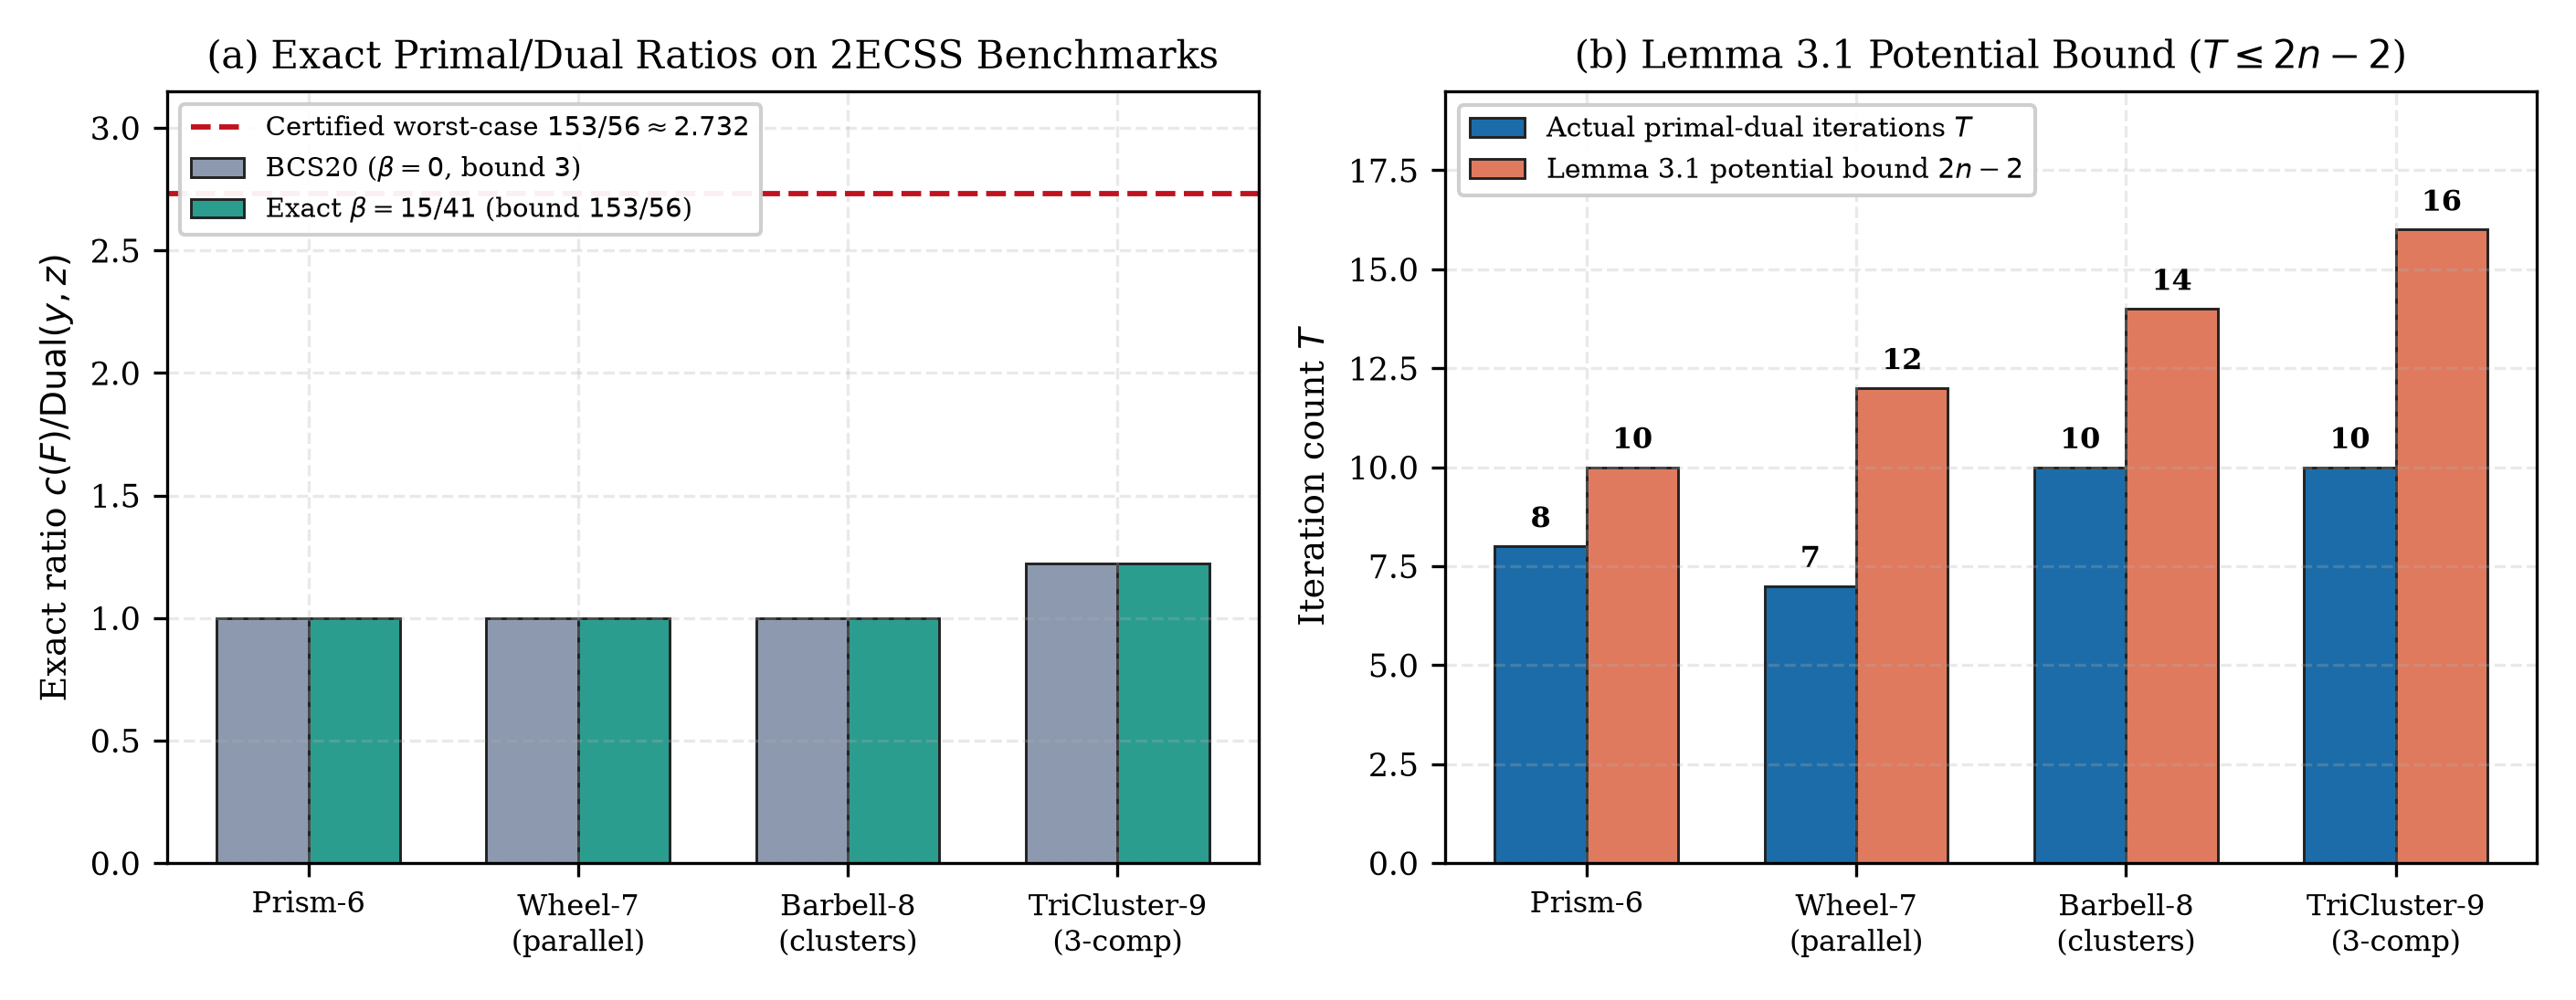
\includegraphics[width=\columnwidth]{figures/fig2_empirical_ratios_and_iters.png}
\caption{(a)~Exact primal/dual ratios on four weighted 2ECSS multigraph benchmarks for $\beta = 0$ versus $\beta = 15/41$. (b)~Actual primal-dual iteration counts $T$ versus Lemma~3.1 potential bound $2n - 2$.}
\label{fig:bench}
\end{figure}

\paragraph{3. 16-certificate atlas, brute-force OPT check, and 57-attack suite.}
Table~\ref{tab:atlas} and Figure~\ref{fig:atlas} summarize all 16 canonical certificates, replayed with zero floats in $0.036$--$0.424\,\mathrm{ms}$ (including a tight connected-tree Theorem~1.2 witness hitting $\mathrm{LHS} = \mathrm{RHS} = 4$). In \texttt{tests/test\_suite.py}, exhaustive enumeration of all $2^{11} = 2{,}048$ edge subsets of \texttt{prism6\_weighted} independently certifies exact $\mathrm{OPT} = 18 = \mathrm{Dual}(y,z) = c(F)$, and 57/57 live adversarial forgeries (broken 2-edge-connectivity, redundant edges, inflated duals violating Constraint~3b, cyclic forests, boundary $\beta \in \{0, 1/2\}$, non-decreasing potential traces, forged $\mathrm{earn}_t$ at $\Delta_t = 0$, $|V_H| > n$, $\kappa \neq |I| + |\mathcal{C}|$, and violated step ratios) are rejected with \texttt{PrimalDual2ECSSCertificateError} (\texttt{3 passed in 0.06s}).

\begin{figure}[t]
\centering
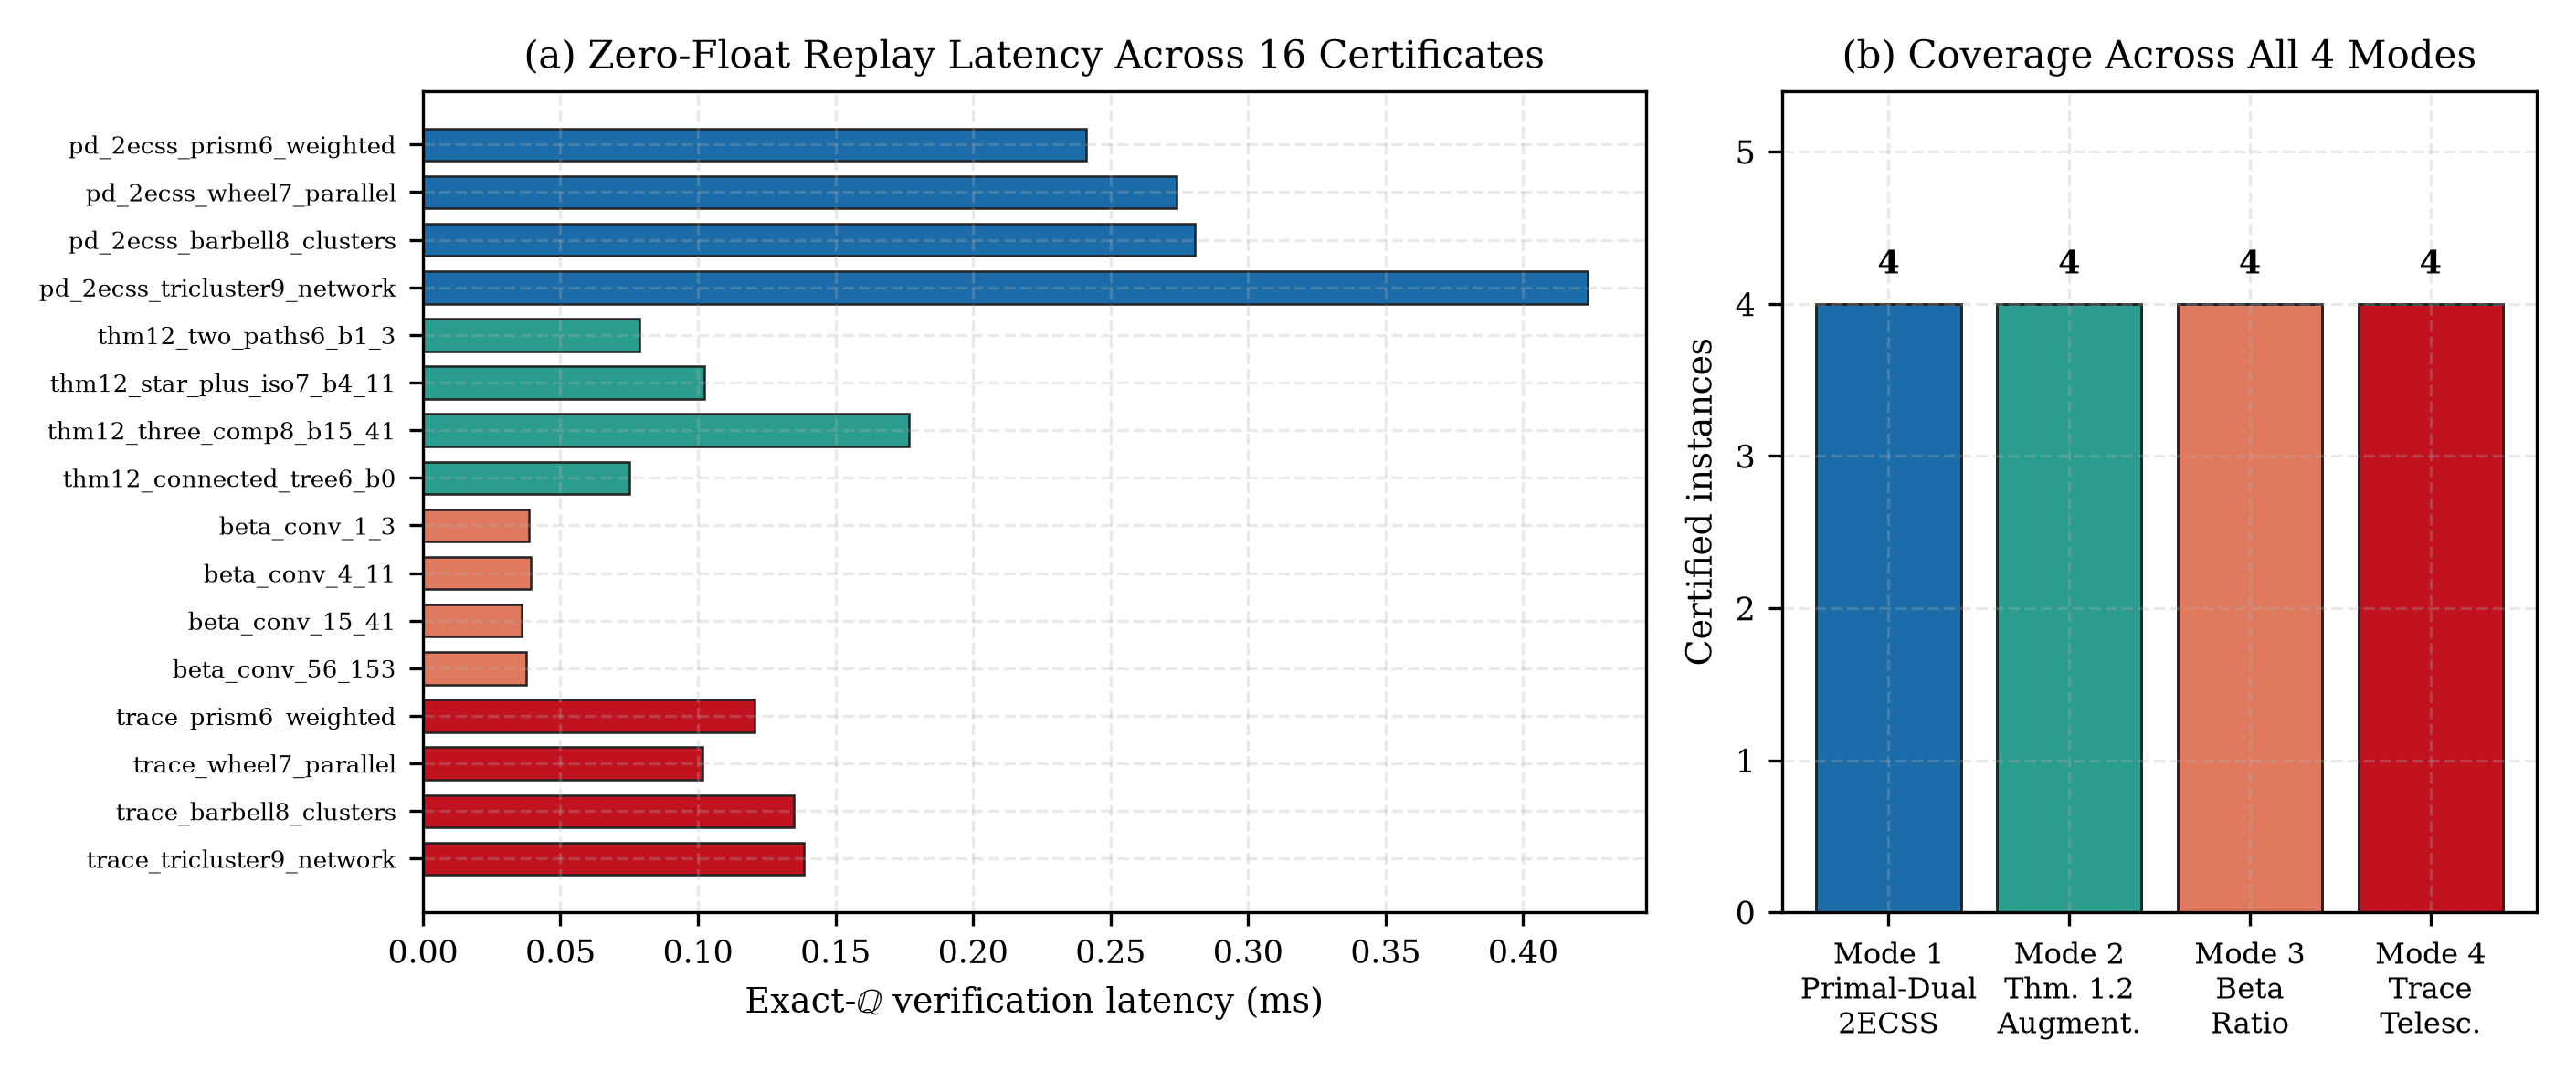
\includegraphics[width=\columnwidth]{figures/fig3_atlas_summary.png}
\caption{(a)~Zero-float replay latency across all 16 canonical \texttt{PRIMAL-DUAL-2ECSS-CERT-1.0} certificates ($0.036$--$0.424\,\mathrm{ms}$). (b)~Balanced 4-per-mode coverage across all four verification modes.}
\label{fig:atlas}
\end{figure}

\begin{table}[t]
\centering
\caption{Summary of all 16 exact-$\QQ$ \texttt{PRIMAL-DUAL-2ECSS-CERT-1.0} certificates (zero floating-point arithmetic; reference-machine replay latency in ms).}
\label{tab:atlas}
\resizebox{\columnwidth}{!}{%
\begin{tabular}{@{}lllr@{}}
\toprule
Certificate File (stem) & Mode & Key Exact Witness & ms \\
\midrule
\texttt{pd\_2ecss\_prism6\_weighted} & M1 & $\beta=1/3,\; c=18,\; D=18\; (\alpha=11/4)$ & 0.241 \\
\texttt{pd\_2ecss\_wheel7\_parallel} & M1 & $\beta=4/11,\; c=25,\; D=25\; (\alpha=41/15)$ & 0.274 \\
\texttt{pd\_2ecss\_barbell8\_clusters} & M1 & $\beta=15/41,\; c=20,\; D=20\; (\alpha=153/56)$ & 0.280 \\
\texttt{pd\_2ecss\_tricluster9\_network} & M1 & $\beta=56/153,\; c=22,\; D=18\; (\alpha=571/209)$ & 0.424 \\
\texttt{thm12\_two\_paths6\_b1\_3} & M2 & $L=4,I=0,C=2,\; 16/3 \le 28/3$ & 0.079 \\
\texttt{thm12\_star\_plus\_iso7\_b4\_11} & M2 & $L=5,I=1,C=2,\; 112/11 \le 194/11$ & 0.102 \\
\texttt{thm12\_three\_comp8\_b15\_41} & M2 & $L=6,I=1,C=3,\; 530/41 \le 918/41$ & 0.177 \\
\texttt{thm12\_connected\_tree6\_b0} & M2 & $L=3,I=0,C=1,\; 4 \le 4$ (tight) & 0.075 \\
\texttt{beta\_conv\_1\_3} & M3 & $\beta=1/3,\; \alpha=11/4,\; \Delta^2=1/16$ & 0.038 \\
\texttt{beta\_conv\_4\_11} & M3 & $\beta=4/11,\; \alpha=41/15,\; \Delta^2=1/225$ & 0.039 \\
\texttt{beta\_conv\_15\_41} & M3 & $\beta=15/41,\; \alpha=153/56,\; \Delta^2=1/3136$ & 0.036 \\
\texttt{beta\_conv\_56\_153} & M3 & $\beta=56/153,\; \alpha=571/209,\; \Delta^2=1/43681$ & 0.038 \\
\texttt{trace\_prism6\_weighted} & M4 & $T=8 \le 10,\; \mathrm{pay}=18,\; \mathrm{earn}=18$ & 0.121 \\
\texttt{trace\_wheel7\_parallel} & M4 & $T=7 \le 12,\; \mathrm{pay}=25,\; \mathrm{earn}=25$ & 0.102 \\
\texttt{trace\_barbell8\_clusters} & M4 & $T=10 \le 14,\; \mathrm{pay}=20,\; \mathrm{earn}=20$ & 0.135 \\
\texttt{trace\_tricluster9\_network} & M4 & $T=10 \le 16,\; \mathrm{pay}=22,\; \mathrm{earn}=18$ & 0.138 \\
\bottomrule
\end{tabular}}
\end{table}

\section{Scope, Limitations, and Conclusion}\label{sec:conclusion}
This work machine-checks the primal-dual ratio algebra, potential termination, weak duality, and telescoping structure of Danciu and Ibrahimpur's better-than-3 2ECSS algorithm~\cite{danciu2026twoconnected}, and provides a zero-float exact-$\QQ$ implementation and sub-millisecond certificate verifier over rational convergents $\beta_k \in (0,1/2)$. It does \emph{not} formalize the general graph-theoretic induction proving Theorem~1.2 over all forests or Theorem~3.5 tight-instance lower bounds in Lean~4, which remain rewarding targets for future graph-theory formalization. Within its verified scope, the combined Lean~4 kernel and \texttt{PRIMAL-DUAL-2ECSS-CERT-1.0} auditor deliver exact, manifest-locked verification for better-than-3 primal-dual 2ECSS solutions.

\bibliographystyle{plain}
\bibliography{references}
\end{document}
